\chapter{Rough calculations}
\section{Punching shear} 
\begin{verbatim}
import rough_calculations.ng_punzonamiento as punch
\end{verbatim}
\begin{center}
\begin{tabular}{p{3cm}p{9.5cm}}
\multicolumn{2}{l}{{\tt punch.esfuerzoPunzonamiento(qk,A)}} \\
& rough estimation of the load on the slab over a support \emph{(HL.3 num. gordos)}\\
\multicolumn{2}{l}{{\tt punch.punzMaximo(fck,d,a,b)}} \\
& rough estimation of the maximum punching force with no need of reinforcement for punching shear  \emph{(HL.3 num. gordos)}\\
\multicolumn{2}{l}{{\tt punch.armaduraPunz(Vd,fck,d,a,b,h,fyd)}} \\
& rough estimation of the reinforcement for punching shear  \emph{(HL.3 num. gordos)} \\
\end{tabular}
\end{center}

where:
\begin{paramFuncTable}
\qkSlab{} \\
\ASupport{} \\
\fck{}\\
\dEff{of the slab} \\
\abSupport{} \\
\h{of the slab} \\
\fyd{of the reinforcement steel} \\
\end{paramFuncTable}

\subsection{Beam deflections}
\begin{verbatim}
import rough_calculations.flechas_vigas as beamDefl
\end{verbatim}
\begin{center}
\begin{tabular}{p{3cm}p{9.5cm}}
\multicolumn{2}{l}{{\tt beamDefl.deflCantBeamPconcentr(l,EI,P,a)}} \\
& maximum deflection in a cantilever beam with a concentrated load at any point \\
\multicolumn{2}{l}{{\tt beamDefl.deflCantBeamQunif(l,EI,q)}} \\
& maximum deflection in a cantilever beam with a uniformly distributed load\\
\multicolumn{2}{l}{{\tt beamDefl.deflCantBeamMend(l,EI,M)}} \\
& maximum deflection in a cantilever beam with a couple moment at the free end\\
\multicolumn{2}{l}{{\tt beamDefl.deflSimplSupBeamPconcentr(l,EI,P,b)}} \\
& maximum deflection in a  beam simply supported at ends with a concentrated load at any point\\
\multicolumn{2}{l}{{\tt beamDefl.deflSimplSupBeamQunif(l,EI,q)}} \\
& maximum deflection in a beam simply supported at ends with a uniformly distributed load\\
\multicolumn{2}{l}{{\tt beamDefl.deflSimplSupBeamMend(l,EI,M)}} \\
& maximum deflection in a beam simply supported at ends with a couple moment at the right end\\
\end{tabular}
\end{center}

\begin{paramFuncTable}
\lSpan{} \\
\EI{} \\
\Pload{} \\
\qload{} \\
\Mcoup{} \\
a & distance from the left end of the beam \\
b & distance from the right end of the beam \\
\end{paramFuncTable}

\clearpage
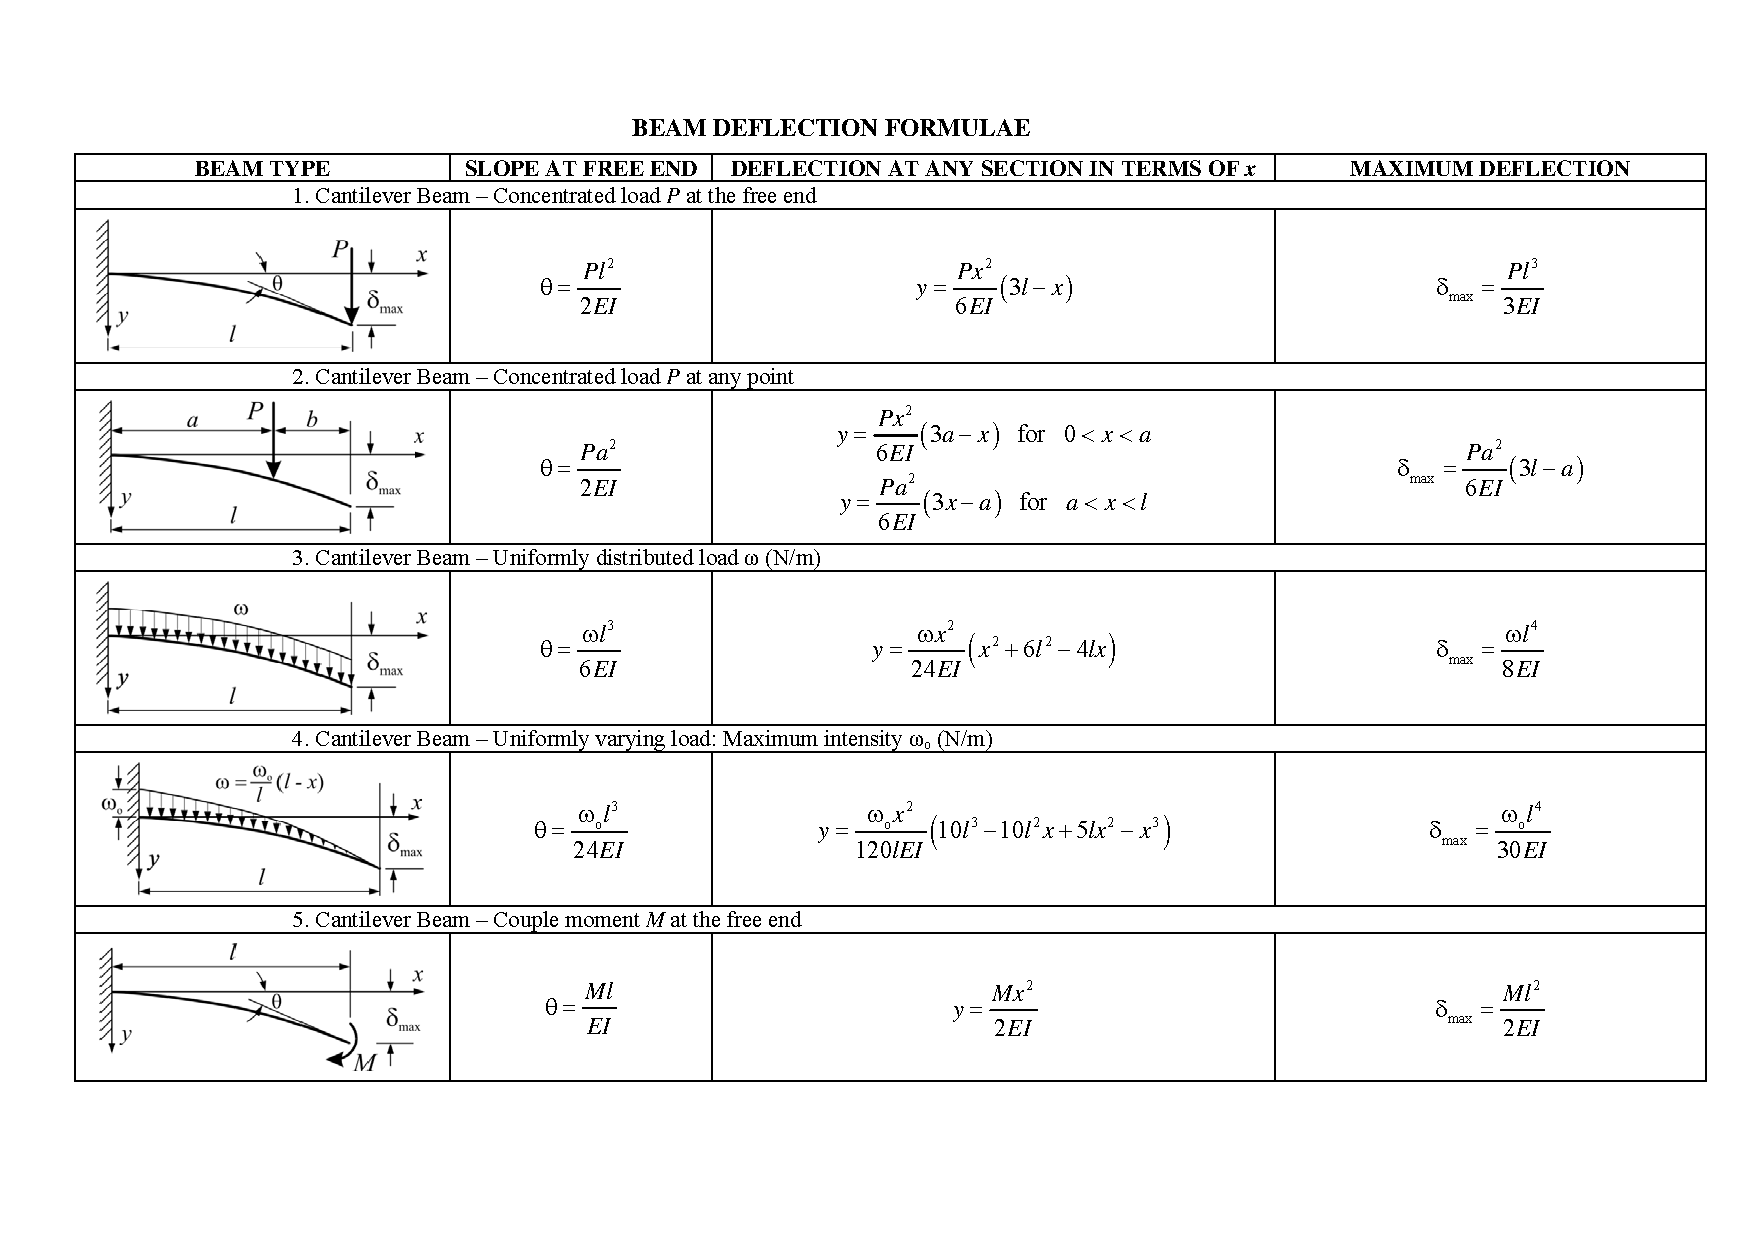
\includepdf[pages={1-2}]{roughCalculations/figures/BeamFormulas.pdf}
